\documentclass[a4paper]{article}

\RequirePackage{graphicx}
\usepackage{authblk}
\usepackage{cleveref}
\usepackage{caption}
%\usepackage{subcaption}
\usepackage[UKenglish]{babel}
\usepackage{alltt}
\usepackage{afterpage}
\usepackage[text={16cm,25cm},centering]{geometry}

%\geometry{
%  a4paper,%
%  top=3cm,%
%  textwidth=16cm,% 
%  textheight=23.2cm,%
%  marginparsep=7pt,% 
%  marginparwidth=2.5cm%
%}

\renewcommand*{\familydefault}{\sfdefault}

\title{Summary of 18th/19th May 2015 Readout System Meeting in Bristol}
\author[1]{Wim Beaumont}
\author[2]{David Cussans}
\author[2]{David Newbold}
\author[3]{Nick Ryder}
\author[3]{Alfons Weber}
\affil[1]{Universiteit Antwerpen}
\affil[2]{University of Bristol}
\affil[3]{University of Oxford}

\date{\today\\V0.0}


\begin{document}


\maketitle

\abstract{
A meeting was held on the 18th/19th of May, 2015, to discuss the readout design for the full SoLid detector.
A proposal for a system level design was agreed.
A number of options for detector parameters were identified.
The collaboration will have to decide on certain parameters soon.
The impact that these decisions will have on the readout system are explained.
A plan for the readout system development is proposed.
}

\tableofcontents

\section{System level design}

\section{Sensor choice}

\section{Amplification and shaping}

\section{Digitisation}

\section{Firmware based trigger}

\subsection{Maximum signal rate for zero suppression}

Each channel's buffer for the zero suppressed data must fit within a single 4608 byte RAM block.
It is assumed that 24 bytes will be stored for each significant EM signal: 4 bytes for timing information and 10 samples each requiring 2 bytes.
A neutron signal will store timing information and 100 samples, requiring 104 bytes.
Each buffer must be able to store a neutron signal and as many significant signals as are needed to contain the IBD analysis time window of $500 \mu$s.
The size of the RAM block ($S_b$) therefore puts a limit on the rate of significant signals, $R_s$
\begin{eqnarray}
    S_b &\ge& S_n + \Delta t_{IBD}\times R_s \times S_s \\
    R_s &\le& (S_b - S_n) / (\Delta t_{IBD} \times S_s)\\
    R_s &\le& 375\mbox{ kHz}
\end{eqnarray}

Since the signal rate in fact fluctuates a safety margin is needed to ensure that all required signals will still be in the buffer at the time of a trigger, and so a target rate of $R_s = 200$ kHz is required.

The aim of the readout system will be to keep all signals from the SiPMs in the zero suppressed buffer, ie using a zero suppression threshold below a single pixel avalanche level.

At low thresholds the dominating signal seen by the SiPMs comes from the high dark count rate.
For the S12572-050C MPPCs used in SM1 the dark count rate (for single pixel avalanches, at $25^{\circ}$C) is typically 1 MHz and maximally 2 MHz.
Other sensors have lower dark count rates, although generally they are above the 200 kHz target rate.
The dark count can also give multi pixel avalanches due to the cross talk between pixels, which ranges from 5\% to 45 \% depending upon the over voltage.
The dark count rate at a level of $n$ photons can be approximated as
\begin{equation}
    R_d(n) = R_d(0)\times C^n,
\end{equation}
with a cross talk probability of $C$.

A range of techniques are available for reducing the signal rate due to dark counts.
The simplest method is to raise the zero suppression threshold.
The firmware will have a programmable zero suppression threshold that can be set at run time.
However this option both reduces the dark count rate and also loses low intensity physical signals, such as those from 511 keV positron annihilation $\gamma$s.

Another method to reduce the signal rate due to dark counts is to require a coincidence between multiple sensors.
In a detector design with a single sensor per row of scintillator cubes a coincidence between at least one vertical and at least one horizontal row can be made.
The signals due to dark counts are then reduced to the rate of accidental coincidences between a vertical and a horizontal row, while real scintillation signals are expected to always give a signal on horizontal and vertical fibres.
The coincidence rate can be estimated as the produce of the signals in each sensor, the time window of the coincidence ($\Delta t$) and the number of sensors compared in the coincidence, $n_{SiPM}$.
\begin{equation}
    R_d^{coinc}(n) = (R_d(0)\times C^n)^2\times\Delta t\times n_{SiPM}
\end{equation}
For the full scale SoLid experiment two possible detector dimensions are being considered: $n_{SiPM} = 16$ or $24$.

If the number of sensors per row of cubes is doubled (either by having a SiPM at either end of a single fibre, or two fibres each with a single SiPM) then a coincidence can be required only with the other SiPM in the same row, reducing $n_{SiPM}$ to 1 and giving a more powerful signal rate reduction.

The signal rates in different scenarios can be estimated in order to select a design that sufficiently lowers the signal rate.
\Cref{rates_s12572_30pct} shows the estimated signal rates using the S12572 MPPC with the over voltage suggested by Hamamatsu, which has a 30\% cross talk probability, and operating at $25^{\circ}$C.
The estimated rates are shown as function of the zero suppression threshold and for different coincidence requirements, either no coincidence, or coincidence with $n_{SiPM} = 1, 16\mbox{ or }24.$
At this over voltage and temperature the required rate can only be achieved with a 0.5 PA threshold using multiple SiPMs per row of scintillator cubes.
In a single ended readout scheme a threshold of 2.5 PA is required to sufficiently reduce the dark count rate.

\begin{figure}[hp]
    \begin{center}
        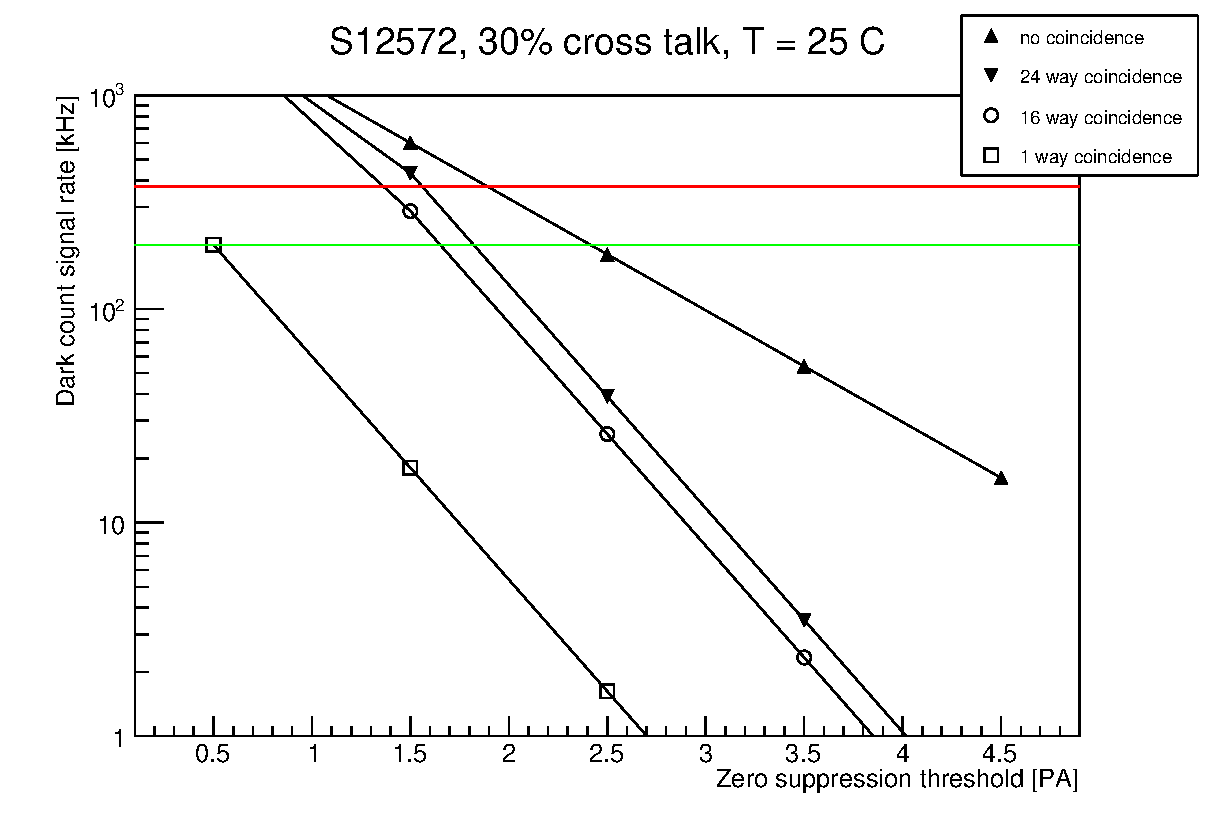
\includegraphics[width=0.8\textwidth]{imgs/g_s12572_30pct}
        \caption{Estimated signal rates for the S12572 MPPC operated with a 30\% cross talk probability.}
        \label{rates_s12572_30pct}
    \end{center}
\end{figure}

Operating the S12572 at a lower over voltage reduces the cross talk probability.
As shown in \cref{rates_s12572_10pct}, operating with an over voltage that reduces the cross talk to 10\% in a single ended readout scheme can allow a 1.5 PA threshold to sufficiently reduce the signal rate.

\begin{figure}[hp]
    \begin{center}
        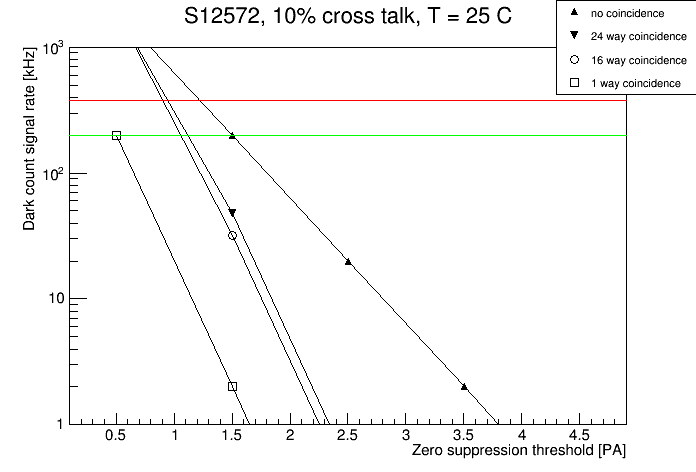
\includegraphics[width=0.8\textwidth]{imgs/g_s12572_10pct}
        \caption{Estimated signal rates for the S12572 MPPC operated with a 10\% cross talk probability.}
        \label{rates_s12572_10pct}
    \end{center}
\end{figure}

The sensl SiPMs may have a reduced dark count rate.
The estimated signal rates for a C Series SiPM are shown in \cref{rates_sensl_10pct}, operating with a 10\% cross talk probability at $21^{\circ}$C.
Again, a threshold of 1.5 PA is required in a single ended readout scheme.

\begin{figure}[hp]
    \begin{center}
        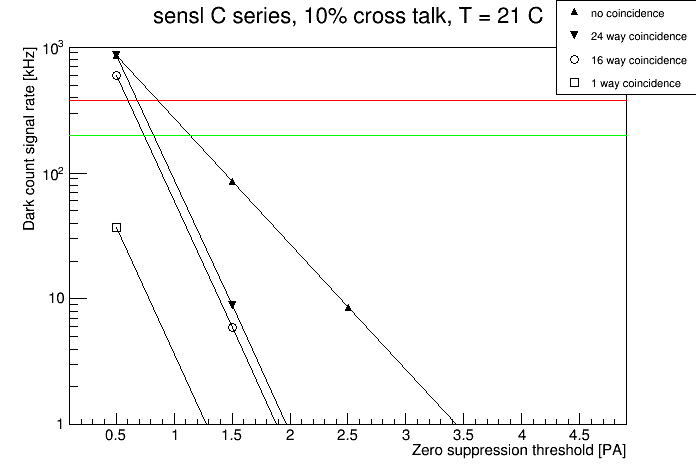
\includegraphics[width=0.8\textwidth]{imgs/g_sensl_10pct}
        \caption{Estimated signal rates for the Sensl C series SiPM operated with a 10\% cross talk probability.}
        \label{rates_sensl_10pct}
    \end{center}
\end{figure}

The dark count rate of a SiPM is highly dependant upon the temperature of operation.
By cooling the sensors the rate can be reduced, leading to a dramatic reduction in the coincidence rate.
\Cref{rates_s12572_10pct_5C} shows the reduction in estimated rates by cooling the S12572 MPPC to $5^{\circ}$C, allowing a 0.5 PA threshold even with a $24\times24$ cube system with single ended readout.
Cooling the SiPMs would require changes to the mechanical design of the detector, but would allow zero suppression with no loss of scintillation signals without the additional cost of doubling the number of sensors per detector volume.

\begin{figure}[hp]
    \begin{center}
        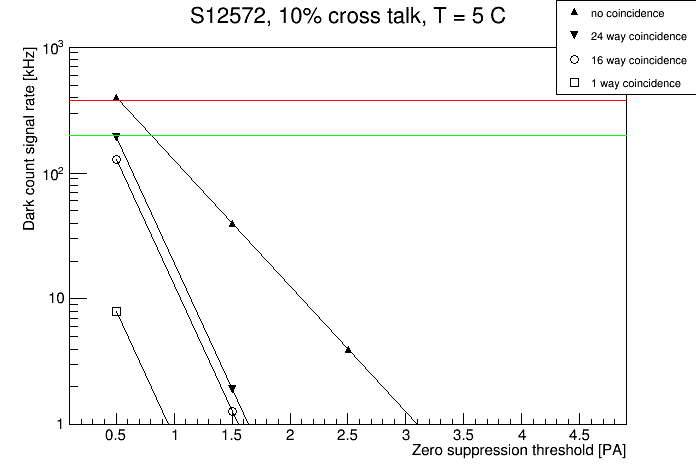
\includegraphics[width=0.8\textwidth]{imgs/g_s12572_10pct_5C}
        \caption{Estimated signal rates for the S12572 MPPC operated with a 10\% cross talk probability cooled to $5^{\circ}$C.}
        \label{rates_s12572_10pct_5C}
    \end{center}
\end{figure}

\section{Software based data reduction}

\section{Readout system development plan}

\end{document}
